\documentclass[10pt]{article}

\usepackage[utf8]{inputenc}
\usepackage[T1]{fontenc}
\usepackage[icelandic,english]{babel}
\usepackage{cancel}
\usepackage{fancyhdr}
\usepackage{float}
\usepackage{hyperref}
\usepackage{wrapfig}
\usepackage{feyn}
\usepackage{units}
\usepackage{siunitx}
\usepackage{gensymb}
\usepackage{textcomp}
\usepackage{tikz}
\usepackage{caption}
\usepackage{subcaption}
\usepackage{enumerate}
\usepackage[shortlabels]{enumitem}
\usepackage{verbatim}

\usepackage{lscape}
\usepackage{rotating}


% ***********************************************************
% ******************* PHYSICS HEADER ************************
% ***********************************************************
% Version 2
\usepackage{amsmath} % AMS Math Package
\usepackage{amsthm} % Theorem Formatting
\usepackage{amssymb}	% Math symbols such as \mathbb

\usepackage{graphicx} % Allows for eps images



%\makeatletter

\usepackage{multicol} % Allows for multiple columns
\usepackage[dvips,letterpaper,margin=0.75in,bottom=0.5in]{geometry}
 % Sets margins and page size
%\pagestyle{empty} % Removes page numbers
\makeatletter % Need for anything that contains an @ command 
\renewcommand{\maketitle} % Redefine maketitle to conserve space
{ \begingroup \vskip 10pt \begin{center} \large {\bf \@title}
	\vskip 10pt \large \@author \hskip 20pt \@date \end{center}
  \vskip 10pt \endgroup \setcounter{footnote}{0} }
\makeatother % End of region containing @ commands
\renewcommand{\labelenumi}{(\alph{enumi})} % Use letters for enumerate
% \DeclareMathOperator{\Sample}{Sample}
% Declare statistical operators
\DeclareMathOperator{\Expect}{E}
\DeclareMathOperator{\Variance}{Var}
\DeclareMathOperator{\Covariance}{Cov}
\DeclareMathOperator{\Correlation}{Corr}

\newcommand{\E}[1]{\Expect \left[ #1 \right]}
\newcommand{\var}[1]{\Variance \left[ #1 \right]}
\newcommand{\cov}[1]{\Covariance \left[ #1 \right]}
\newcommand{\corr}[1]{\Corelation \left[ #1 \right]}
\newcommand{\s}[1]{\sigma_{#1}}



\DeclareMathOperator{\GINI}{\text{Gini}}
\newcommand{\gini}[1]{\GINI \left( \text{#1} \right)}
\DeclareMathOperator{\Entropy}{\text{Entropy}}
\newcommand{\entropy}[1]{\Entropy \left( \text{#1} \right)}
\DeclareMathOperator{\Gain}{\text{Gain}}
\newcommand{\gain}[1]{\Gain \left( \text{#1} \right)}
\DeclareMathOperator{\ErrorRate}{\text{Error}}
\newcommand{\error}[1]{\ErrorRate \left( \text{#1} \right)}




\let\vaccent=\v % rename builtin command \v{} to \vaccent{}
\renewcommand{\v}[1]{\ensuremath{\mathbf{#1}}} % for vectors
\newcommand{\gv}[1]{\ensuremath{\mbox{\boldmath$ #1 $}}} 
% for vectors of Greek letters
\newcommand{\uv}[1]{\ensuremath{\mathbf{\hat{#1}}}} % for unit vector
\newcommand{\abs}[1]{\left| #1 \right|} % for absolute value
\newcommand{\avg}[1]{\left< #1 \right>} % for average
\let\underdot=\d % rename builtin command \d{} to \underdot{}
\renewcommand{\d}[2]{\frac{d #1}{d #2}} % for derivatives
\newcommand{\dd}[2]{\frac{d^2 #1}{d #2^2}} % for double derivatives
\newcommand{\pd}[2]{\frac{\partial #1}{\partial #2}} 
% for partial derivatives
\newcommand{\pdd}[2]{\frac{\partial^2 #1}{\partial #2^2}} 
% for double partial derivatives
\newcommand{\pdc}[3]{\left( \frac{\partial #1}{\partial #2}
 \right)_{#3}} % for thermodynamic partial derivatives
\newcommand{\ket}[1]{\left| #1 \right>} % for Dirac bras
\newcommand{\bra}[1]{\left< #1 \right|} % for Dirac kets
\newcommand{\braket}[2]{\left< #1 \vphantom{#2} \right|
 \left. #2 \vphantom{#1} \right>} % for Dirac brackets
\newcommand{\matrixel}[3]{\left< #1 \vphantom{#2#3} \right|
 #2 \left| #3 \vphantom{#1#2} \right>} % for Dirac matrix elements
\newcommand{\grad}[1]{\gv{\nabla} #1} % for gradient
\let\divsymb=\div % rename builtin command \div to \divsymb
\renewcommand{\div}[1]{\gv{\nabla} \cdot #1} % for divergence
\newcommand{\curl}[1]{\gv{\nabla} \times #1} % for curl
\let\baraccent=\= % rename builtin command \= to \baraccent
\renewcommand{\=}[1]{\stackrel{#1}{=}} % for putting numbers above =
\newtheorem{prop}{Proposition}
\newtheorem{thm}{Theorem}[section]
\newtheorem{lem}[thm]{Lemma}
\theoremstyle{definition}
\newtheorem{dfn}{Definition}
\theoremstyle{remark}
\newtheorem*{rmk}{Remark}


% ***********************************************************
% ********************** END HEADER *************************
% ***********************************************************

% Easier commands for matrices
\newcommand{\bpm}{\begin{pmatrix}}
\newcommand{\epm}{\end{pmatrix}}

\newcommand{\bvm}{\begin{vmatrix}}
\newcommand{\evm}{\end{vmatrix}}

\newcommand{\bbm}{\begin{bmatrix}}
\newcommand{\ebm}{\end{bmatrix}}

\newcommand{\texttip}[2]{#1}


% Easier commands for typical multivariate random variables
\newcommand{\X}{\mathrm{X}}
\newcommand{\Y}{\mathrm{Y}}
\newcommand{\Z}{\mathrm{Z}}

% Questions are often divided into sections (a,b,c...etc), this custom command creates sort of a subsubsub-section for these.
\newcommand{\questi}[1]{\vspace{0.45cm}\textbf{#1}\vspace{0.25cm}\\}


\title{\Huge REI502M - Introduction to Data Mining\\  \Large Report on Project 1}
\author{Elías Snorrason}

\setcounter{section}{0}
\setcounter{secnumdepth}{2}

\begin{document}

% Following is a renewed commands for the subsection and subsubsection to make the spacing more comfortable. This is also how the \smallbosonloop diagram is added to each question.
\makeatletter
\renewcommand\subsubsection{\@startsection{subsubsection}{3}{\z@}%
{-3.25ex\@plus -1ex \@minus -.2ex}%
{1.5ex \@plus .2ex}%
{\small{$\smallbosonloopV \quad $} \quad \normalfont\large\bfseries\emph}}% 

\renewcommand\subsection{\@startsection{subsection}{2}{\z@}%
{-3.25ex\@plus -1ex \@minus -.2ex}%
{2.5ex \@plus .2ex}%
{\normalfont\large\bfseries}}% 
\makeatother

\quad
\vspace{3cm}
\maketitle
\setcounter{page}{1}
\thispagestyle{fancy}
%\lhead[rh-even]{Student:\\ \textbf{Elías Snorrason}}
%\rhead[lh-even]{Teacher:\\ \textbf{Nikolay Gagunashvili}}

\hrule
\tableofcontents
\newpage


\vspace{3cm}
%\begin{center}
%\includegraphics[width=0.45\textwidth]{Haskoli_Islands_rett.jpg}
%\end{center}


\section{Pre-processing}

\begin{itemize}
\item The data set can be found in an arff format at \\ \href{github.com/ongxuanhong/Preprocessing-with-horse-colic-dataset/blob/master/horse-colic.arff}{https://github.com/ongxuanhong/Preprocessing-with-horse-colic-dataset/blob/master/horse-colic.arff}
\end{itemize}
The data set we have chosen is in the field of veterinary. More specifically, horse health. Successful association rule mining could potentially help veterinarians with diagnosis and  to evaluate treatment.\\
We start by having a look at the data through the visualize tab in Weka.
\begin{figure}[h!]
\centering
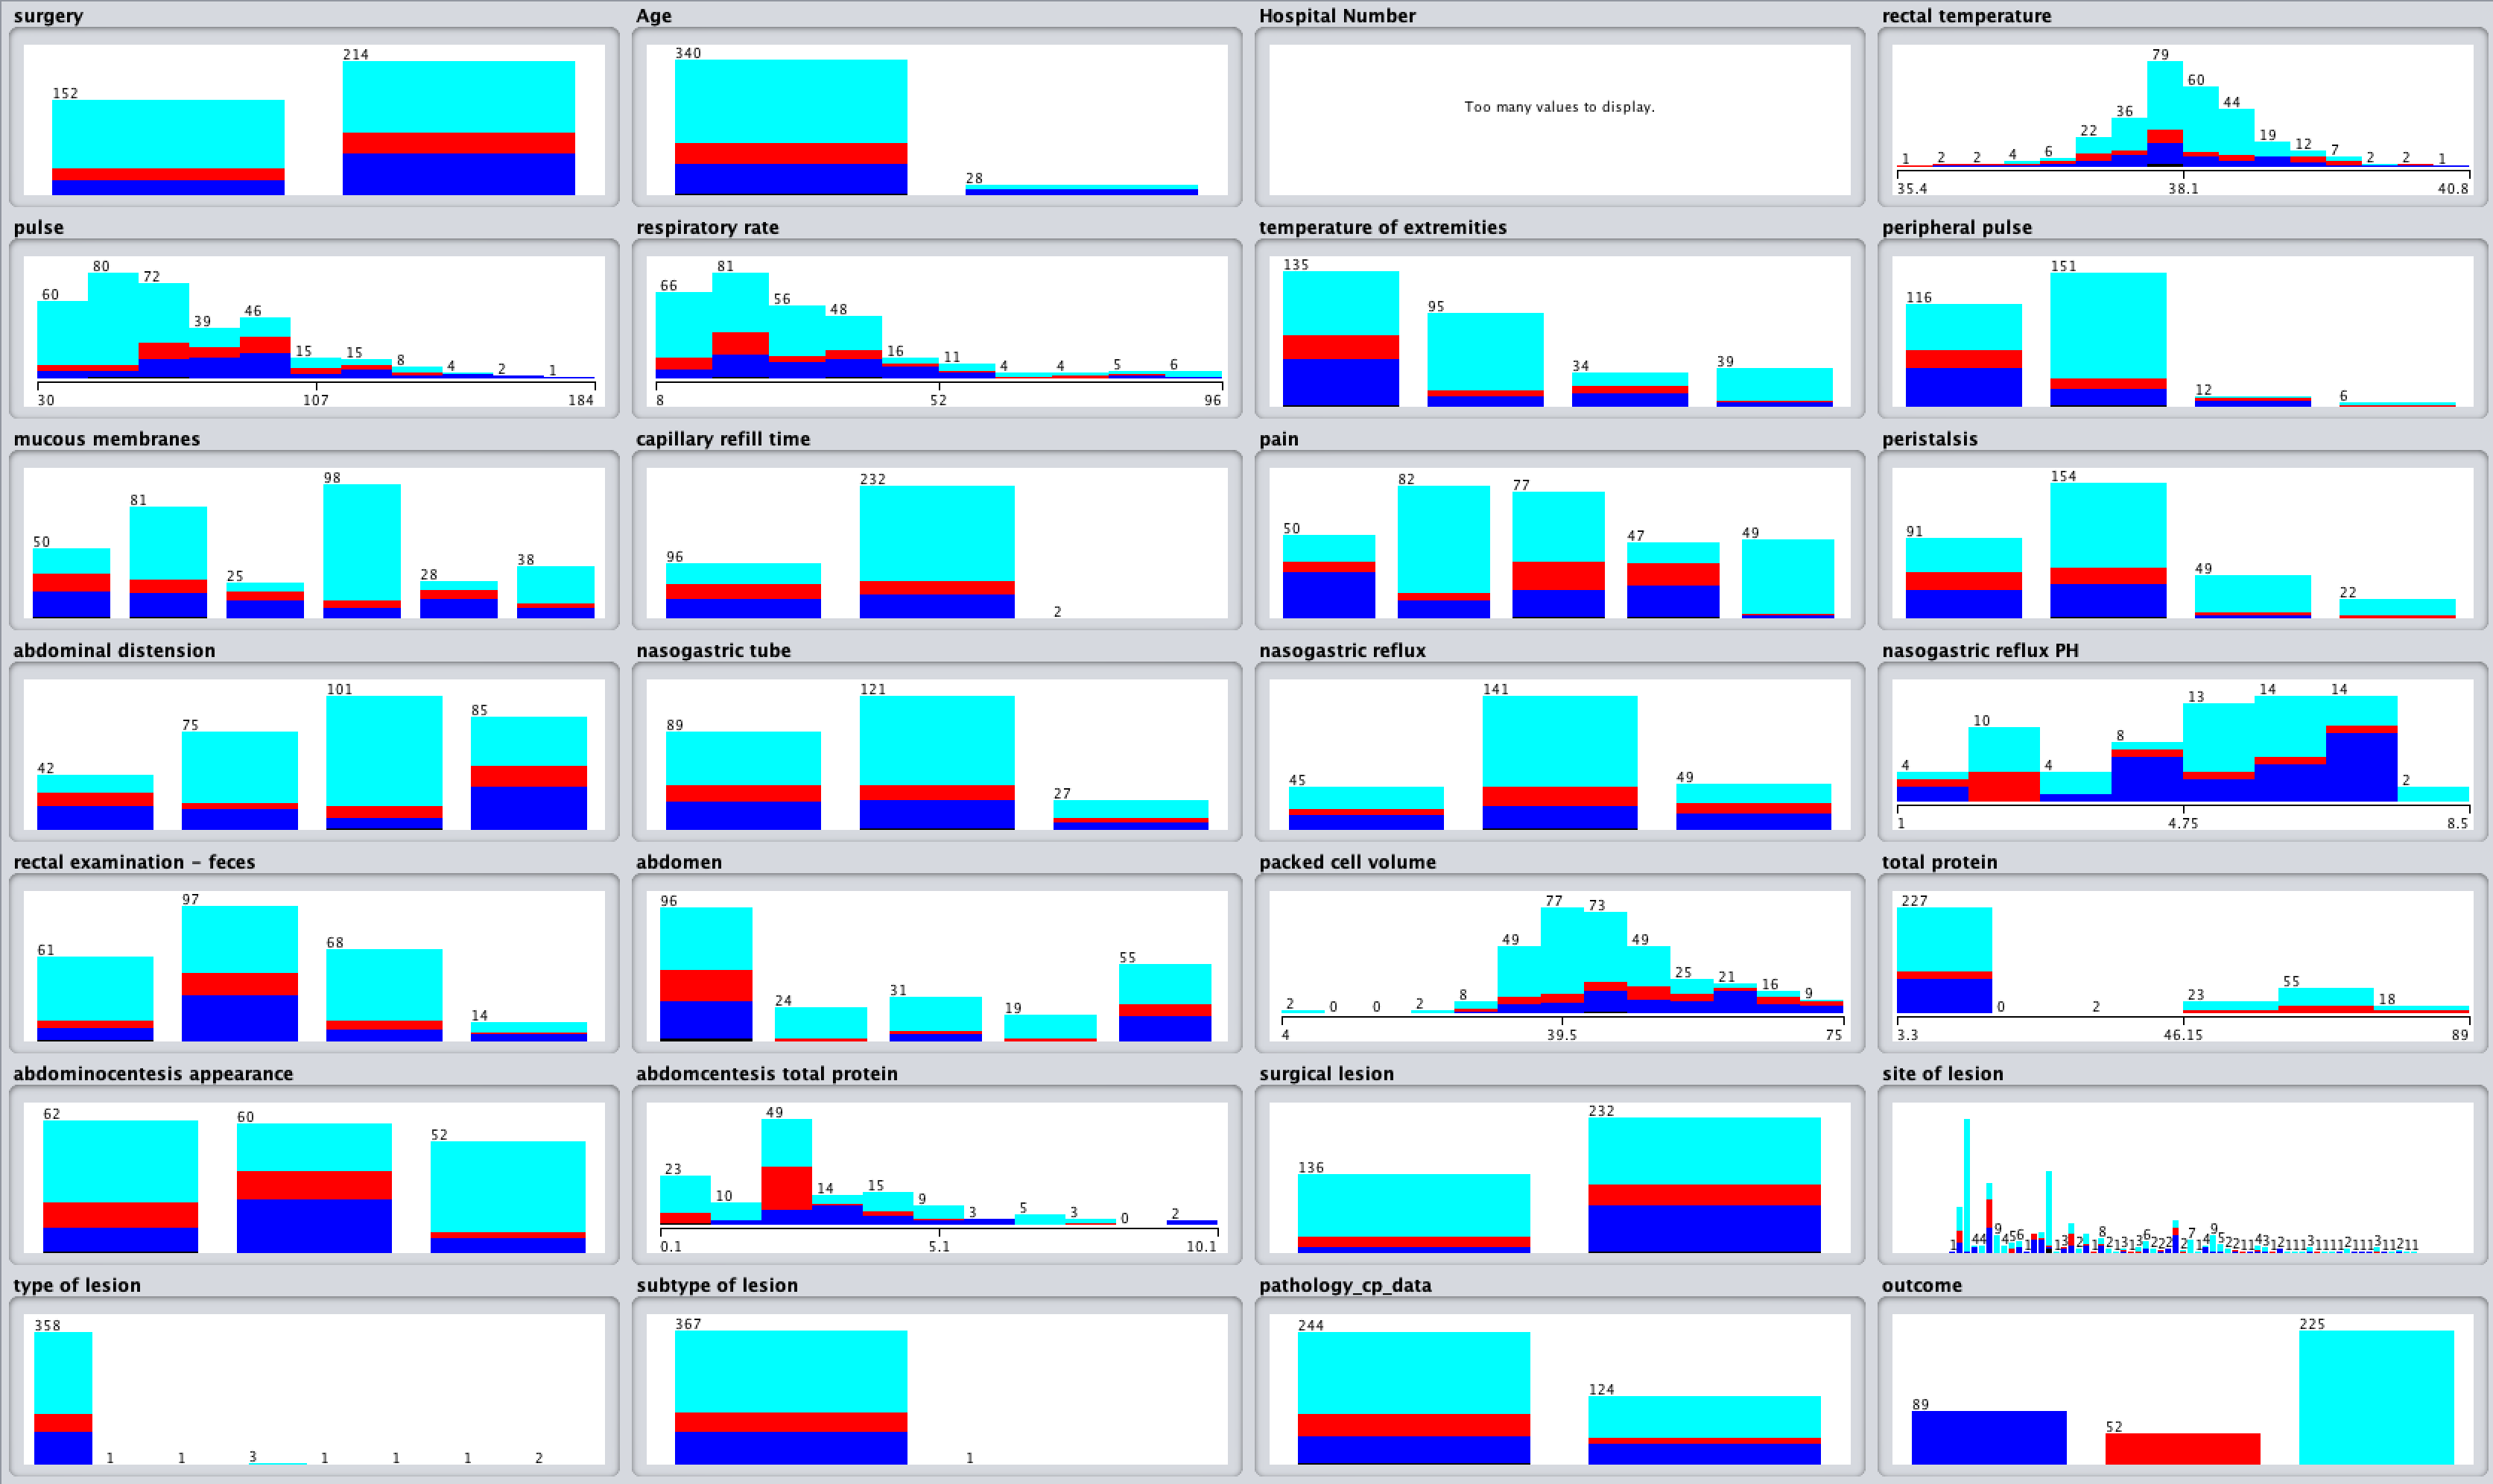
\includegraphics[width=17cm]{originalAttributeDistribution}
\caption{The original attribute value distribution}
\end{figure}

As we can see the attributes: Age, Type of lesion and Subtype of lesion are very unevenly distributed. So we remove them along with the attribute pathology$\_$cp$\_$data. That attribute was described as being unsignificant in the attribute information sheet.
In order to use the Apriori algorithm the all attributes have to be nominal. So we discretize the following attributes accordingly. Our objective in that sense is to find some interesting rules with relatively low support but high confidence.
We set the \verb|outcome| as the new class value. Even though association rule mining does not rely on classes  \verb|outcome| could be an interesting metric in the case of using association rule mining for classification. \\\\
\begin{itemize}
The outcome values are renamed as:
\begin{itemize}
\item lived
\item died
\item was euthanized
\end{itemize}

\item The rectal temperature was discretized to throw out extreme values, using 8 bins.

\item The pulse attribute was also discretized, this time into 8 bins with equal frequency.

\item The respiratory rate was relabeled accordingly:
\begin{itemize}
\item Normal: 8-10 bpm
\item Above Normal: 11-25 bpm
\item Fast: 26-35 bpm
\item Extreme: Over 35 bpm
\end{itemize}

\item Total protein was discretized into 5 bins
\begin{itemize}
\item < 5.5 gms/dL
\item 5.5-6.4 gms/dL
\item 6.5-7.5 gms/dL
\item 7.6 - 10 gms/dL
\item > 10 gms/dL
\end{itemize}


\item Abdomcentesis total protein was split into 3 bins
\begin{itemize}
\item 0- 1.5 gms/dL
\item 1.6 - 3 gms/dL
\item > 3 gms/dL
\end{itemize}

\item packed cell volume was split into 3 bins
\begin{itemize}
\item < 31 \%
\item 31-50 \%
\item > 50 \%
\end{itemize}

\item nasogastric reflux pH was split into 3 bins


\end{itemize}

Note: Using the \verb|MergeManyValues| for numerical attribues...

\subsection{Determining upper and lower bound support}

Because the total number of possible rules extracted
from a data set grows exponentially it is necessary to find a minimum support count so we don't have to waste computational power in finding uninteresting and obvious rules.
We want to find rules with relatively low support and high confidence.
We run the apriori algorithm and let weka generate output itemsets for us.  We copy the one itemset frequency list into excel and generate the following table.


\begin{figure}[H]
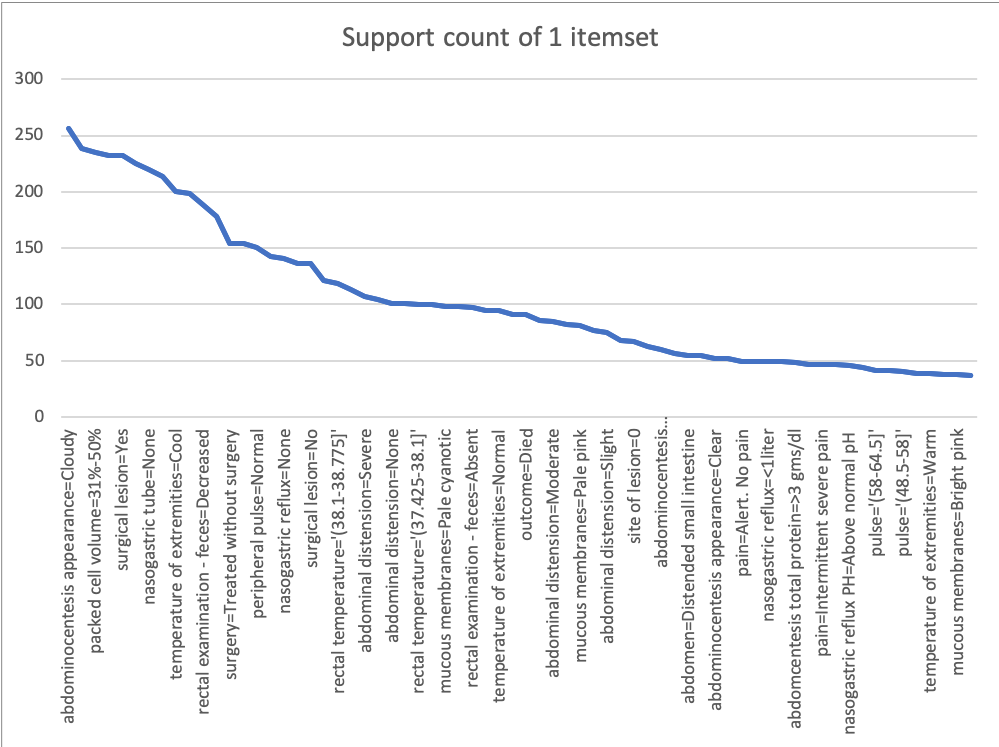
\includegraphics[scale=0.7]{SupportCountTable.png}

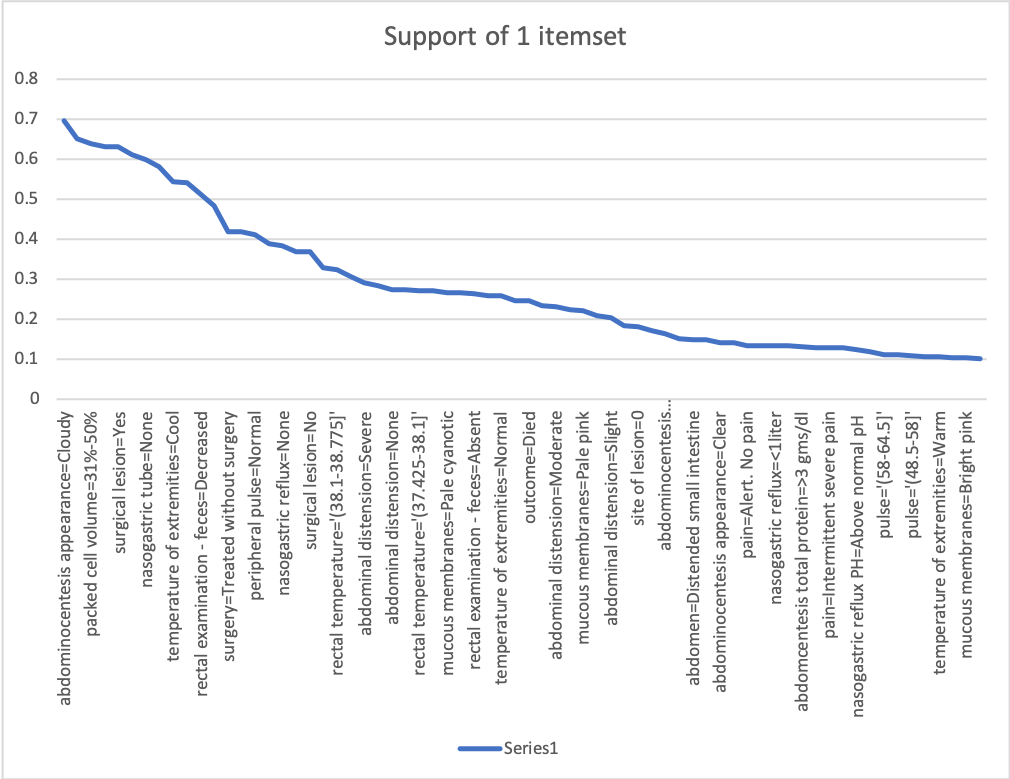
\includegraphics[scale=0.7]{SupportTable.png}
\end{figure}

We deduct from the table that the most interesting rules will have support level of less than 0.42 since any rule with more support than that will probably be rather obvious. So we set the upperBoundMinSupport to 0.42 in the Associate settings.\\
Since there are no itemset with support lower than 0.1 we can set the lowerBoundMinSupport to 0.1.
\section{Metric-based rule selection}

After removing uneven attributes and discretizing all of the numerical attributes in our data set, we can investigate the rules generated by the Apriori algorithm. 

We have 4 potential metrics for ranking our rules.
\begin{itemize}
\item Confidence
\item Lift
\item Leverage
\item Conviction
\end{itemize}
%
\subsection{Confidence}
Setting a threshold for this metric ($minconf = 0.95$) results in hundreds of high confidence rules.
E.g. running 
\begin{verbatim}
	   weka.associations.Apriori -I -R -N 1000 -T 0 -C 0.95 -D 0.05 -U 1.0 -M 0.1 -S -1.0 -c 24
\end{verbatim}

\begin{itemize}

\item \verb|95. surgery=Treated without surgery |

\verb|peripheral pulse=Normal| 

\verb|site of lesion=0| 

\verb|outcome=Lived 39| 

\verb|   ==>|

\verb|surgical lesion=No 39|

\verb|<conf:(1)> lift:(2.71) lev:(0.07) [24] conv:(24.59)|

%%%%%
%%%%%

\item \verb|105. peristalsis=Absent,|

\verb|abdominal distension=Severe,|

\verb|nasogastric reflux=>1liter,|

\verb|rectal examination - feces=Decreased 39|

\verb|   ==>|

\verb|abdomen=Distended lg intestine 39|

\verb|<conf:(1)> lift:(1.54) lev:(0.04) [13] conv:(13.67)|

%%%%%
%%%%%

\item \verb|844. capillary refill time=<3sec,|

\verb|abdominocentesis appearance=Cloudy,|

\verb|site of lesion=0 40| 

\verb|   ==>|

\verb|surgical lesion=No ,|

\verb|outcome=Lived 38|

\verb|<conf:(0.95)> lift:(3.21) lev:(0.07) [26] conv:(9.38)|
\end{itemize}
%
The first rule can be considered as an obvious rule (non-existing lesions don't require surgical intervention).
However, the next rule has identical support and confidence and can be useful in a diagnostic sense.
The last rule can potentially help with making a prognosis (in select few cases).


\subsection{Lift}
We get 460 rules when we set $minlift = 4.0$ and run
\begin{verbatim}
	  weka.associations.Apriori -I -R -N 1000 -T 1 -C 4.0 -D 0.05 -U 1.0 -M 0.1 -S -1.0 -c 24
\end{verbatim}
With moderately high confidence, we get an interesting rule, which may be suitable for diagnosis:
\begin{itemize}
\item   \verb|8. peripheral pulse=Reduced|

\verb|pain=Continous severe pain| 

\verb|peristalsis=Absent| 

\verb|nasogastric tube=None| 

\verb|abdominocentesis appearance=Cloudy 41 |


\verb|==>| 


\verb|temperature of extremities=Cool| 

\verb|abdominal distension=Severe |

\verb|abdomen=Distended lg intestine 37 | 
  
\verb|conf:(0.9) < lift:(4.68)> lev:(0.08) [29] conv:(6.62)|

\end{itemize}



\subsection{Leverage}
Using this metric (e.g. $minleve = 0.1$) results in multiple rules with obvious correlations between their attributes.
These rules are usually on the form:
\begin{itemize}
\item \verb|2. surgery=Treated without surgery| 

\verb|outcome=Lived 110|


\verb|   ==>|
 
\verb|surgical lesion=No 97|

\verb|conf:(0.88) lift:(2.39) < lev:(0.15) [56]> conv:(4.95)|
\end{itemize}
For this metric to be more useful, we need to remove more attributes from the data set.



\section{Rule generation} \label{sec: rule gen}
After the investigation of minimum support as well as different metrics for rule generation, we remove attributes such as \verb|surgery|, \verb|site of lesion|, \verb|outcome| and \verb|hospital number|. This removes some bias from the data, and allows for more exploratory learning. In this section, \verb|abdomen| is chosen as the class attribute for classification with association rule analysis.

\begin{figure}[H]
\centering
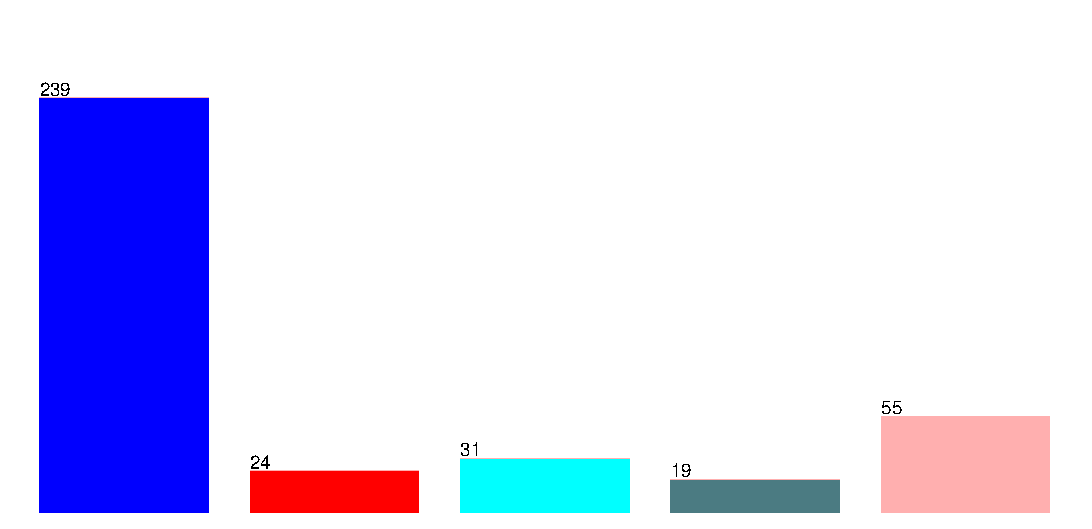
\includegraphics[scale=0.8]{abdomen-class}
\caption{Distribution of the \textit{abdomen}-attribute, with values: distended lg intestine, other, Normal, Firm feces in the lg intestine, Distended small intestine}
\end{figure}

\begin{verbatim}
	weka.associations.Apriori -R -N 1000 -T 0 -C 0.4 -D 0.05 -U 0.42 -M 0.1 -S -1.0 -A -c 20
\end{verbatim}
\begin{itemize}
\item \verb|231. pain=Continous severe|

\verb|pain peristalsis=Absent |

\verb|rectal examination - feces=Decreased |

\verb|abdominocentesis appearance=Cloudy 46|
 
\verb| ==> |

\verb|abdomen=Distended lg intestine 44   |

\verb|conf:(0.96)|
\end{itemize}
\begin{verbatim}
	weka.associations.Apriori -R -N 1000 -T 0 -C 0.95 -D 0.05 -U 0.42 -M 0.1 -S -1.0 -c 20
\end{verbatim}
\begin{itemize}
\item \verb|1. pain=Continous severe pain|

\verb|nasogastric reflux=>1liter |

\verb|abdominocentesis appearance=Cloudy 55|

 \verb| ==> |
 
 \verb|abdomen=Distended lg intestine 55 |

 \verb| <conf:(1)> lift:(1.54) lev:(0.05) [19] conv:(19.28)|
\end{itemize}

\begin{verbatim}
	weka.associations.Apriori -R -N 1000 -T 1 -C 4.0 -D 0.05 -U 0.42 -M 0.1 -S 0.01 -c 20
\end{verbatim}

\begin{itemize}
\item  \verb|21. temperature of extremities=Cool|

\verb|peripheral pulse=Reduced |

\verb|pain=Continous severe pain|

\verb|nasogastric tube=None |

\verb|abdominocentesis appearance=Cloudy 41 |

\verb|==> |

\verb|peristalsis=Absent |

\verb|abdominal distension=Severe |

\verb|abdomen=Distended lg intestine 37    |

\verb|conf:(0.9) < lift:(4.55)> lev:(0.08) [28] conv:(6.57)|
\end{itemize}

%\input{./pre_processing}
%\input{./decision_tree_creation}
%\input{./problems/D3-2}
%\input{./problems/D3-3}
%\input{./problems/D3-5}
%
\newpage

\end{document}
